\section{\emph{RDF Schema}}
Dalam kasus yang lebih kompleks, RDF tidak cukup kuat untuk menjelaskan semantik dari sebuah subjek yang sedang dijelaskan. Jika kita kembali pada contoh di atas, apabila kita ingin lebih jauh menjelaskan mengenai misalnya apa/siapa Syamsul Muttaqin, RDF tidak dapat menjelaskan hal ini \citep*{antoniou}. Untuk mengatasi hal ini, maka di diperkenalkan RDF Schema (RDFS).

\begin{figure}[h]
	\centering
	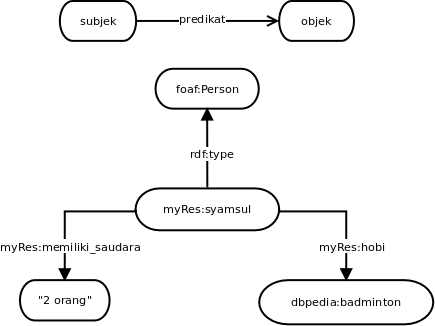
\includegraphics[trim = 0mm 0mm 0mm 32mm, clip, scale=0.55]{gambar}
	\caption{RDFS-statement}
	\label{fig:rdfs_statement}
\end{figure}

Sesuai dengan namanya, RDF Schema memberikan penjelasan lebih jauh mengenai objek yang sedang dibicarakan. Untuk itu RDFS diperkaya dengan beberapa penambahan namespace seperti rdfs:Class yang digunakan untuk menjelaskan tipe dari sebuah objek, rdfs:subClassOf yang merupakan turunan dari kelas, rdfs:domain, rdfs:range, serta beberapa penambahan lainnya. Gambar \ref{fig:rdfs_statement} menunjukkan RDFS statement, dimana \emph{foaf:Person} adalah kelas dan \emph{myRef:syamsul} merupakan \emph{instance} dari kelas \emph{Person}.